%% LyX 2.0.3 created this file.  For more info, see http://www.lyx.org/.
%% Do not edit unless you really know what you are doing.
\documentclass[english]{report}
\usepackage[T1]{fontenc}
\usepackage[utf8]{luainputenc}
\setcounter{secnumdepth}{3}
\setcounter{tocdepth}{3}
\usepackage{graphicx}
\usepackage{babel}
\begin{document}

\title{Assignment 3: Sudoku Orbits}


\author{Justin Miller}

\maketitle

\section*{Purpose}

We want to see how many orbits there are for a given puzzle. On top
of this we are going to try and use openmp Sections and For to help
speed it up. 


\section*{Running}

The command that I use to run it is ./sudoku \$(cat input.txt) > output.txt
\&.

There is MAX\_THREADS for max threads of the computer and can be set
by hand.

There is PARR to decide to run in unique finding mode (0) or parallel
sections (1)


\section*{Calculated Amount}

We find that for each type of change to a puzzle there are
\begin{itemize}
\item Relabel: 9! = 362880
\item Row Permutation: $3!^{3}=216$
\item Band Permutation: $3!=6$
\item Column Permutations: $3!^{3}=216$
\item Pillar Permutations: $3!=6$
\item Rotation Permutations: 4
\item Reflection Permutations: 2
\end{itemize}
Now we see that the combination of row, band, column, pillar, rotation,
and reflection means that rotations = 2 since if we rotate once more
we have just reflected and we see that reflections are not needed
since row and band do the same. Thus we find that
\begin{itemize}
\item Row+Band+Column+Pillar+Rotation Permutations: $3!*3!^{3}*3!*3!^{3}*2=3!^{8}*2=3,359,232$
\end{itemize}
Now we see that if we try and add in relabel we get
\begin{itemize}
\item $3,359,232*9!=1,218,998,108,160$
\end{itemize}
Thus I decided that I will not do that instead I will just add that
relabel and rotation thus I get
\begin{itemize}
\item $3,359,232+9!*2=4,084,992$
\end{itemize}

\section*{Computer Found Amount}

Doing the same thing as the calculated but finding the permutations
and the puzzle that it has found it finds that there are 4,084,992
solutions. We see that the solutions match, which it should.


\section*{Time Improvements}


\subsection*{Section}

The first thing that we are going to try and find the improvements
by putting the code of permutations and relabeling in different sections.
Here we get the chart

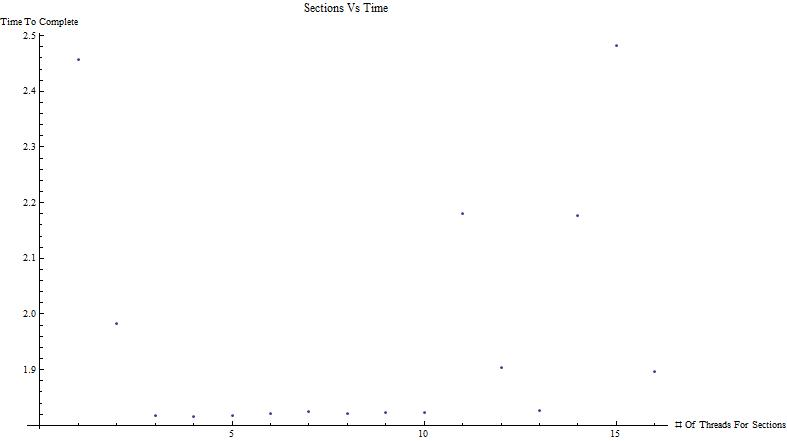
\includegraphics[width=1\columnwidth]{Graph2}

What we see is that it does improve performance but only to 3 threads,
after that the computer doesn't get any improvements and later gets
big overhead.

Finding the best is at threads = 4, and the time is 1.815079 seconds
at an efficiency of 0.7385091553 or 1.35 times faster.


\subsection*{For: Permutations }

The next thing that we want to see is the improvements on using a
openmp For parallel for the permutations section.

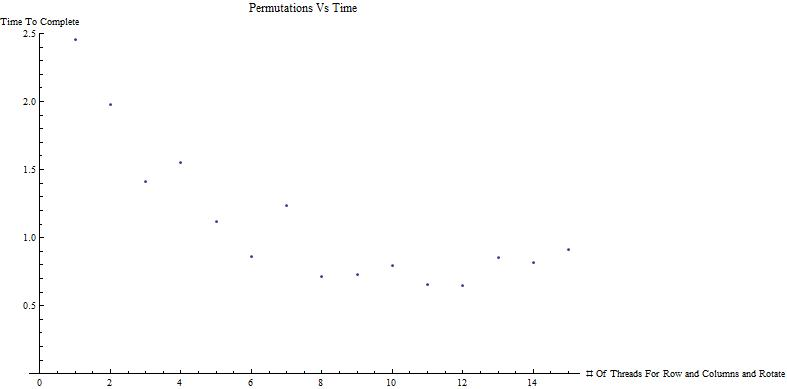
\includegraphics[width=1\columnwidth]{Graph3}

And here we see that it does improve.

Finding the best is at threads = 12, and the time is 0.648182 seconds
at an efficiency of .2637286538 or 3.79 times faster.

This is so far the best improvement.


\subsection*{For: Relabel}

The next thing that we going to find is the best number of threads
for relabel.

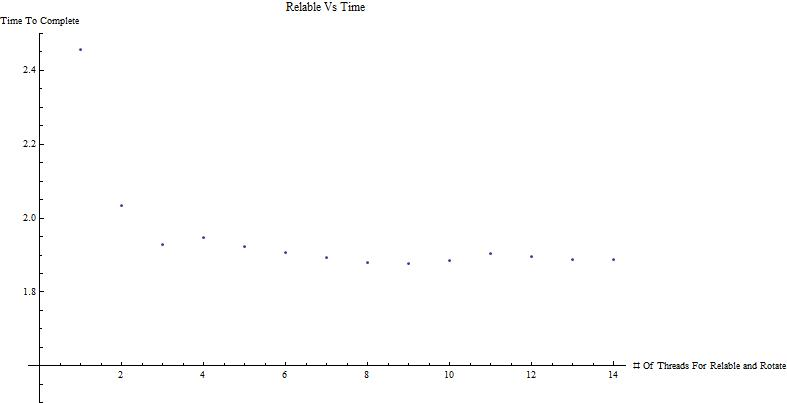
\includegraphics[width=1\columnwidth]{Graph4}

And it also improves.

Finding the best is at threads = 9, and the time is 1.875766 seconds
at an efficiency of 0.7632011412 or 1.31 times faster.

This is the worst optimization so far.


\subsection*{Sections: For: Relabel + For: Permutations }

Now we are going to see what the best combination of all three is.
For the graph we did just For of Relabel and For: Permutations.

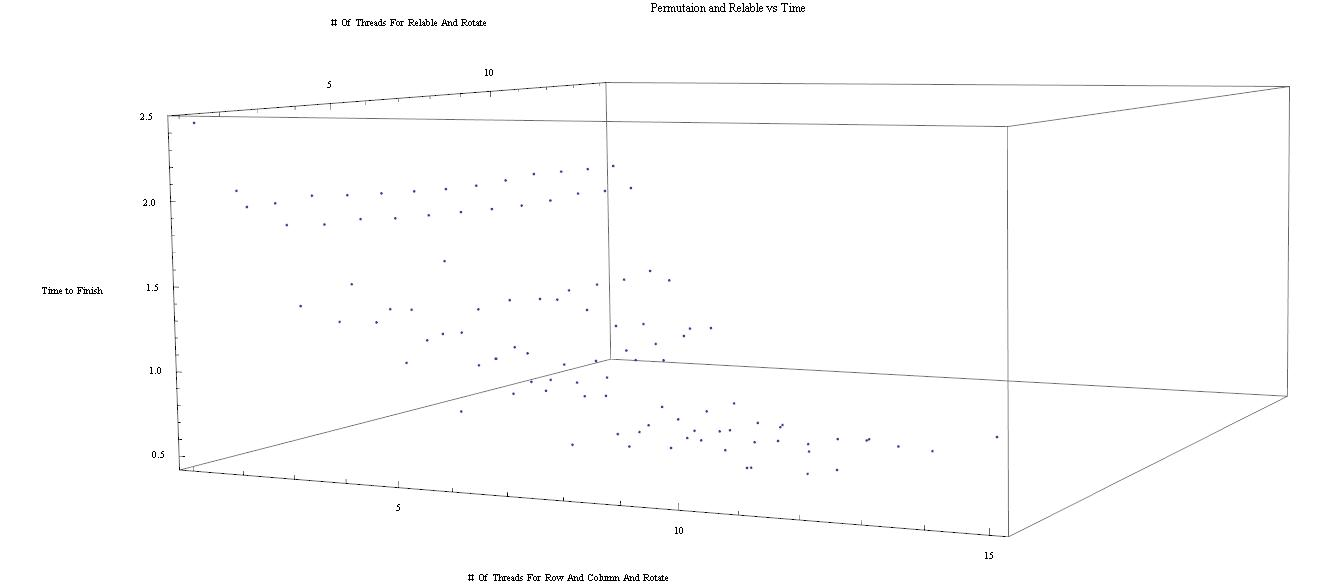
\includegraphics[width=1\columnwidth]{Graph1}

And the best combination that we can find is 1 thread for Sections,
11 Threads for Permutations, and 4 Threads for Relabeling for a time
of 0.458857 or a 5.356267857 speedup knowing from Amdahl's law that
we see that $\frac{\frac{1}{5.356267857}-1}{\frac{1}{14}-1}*100=87.58645963\%$
of the code is paralleled.


\section*{Finding Unique Solutions}


\subsection*{Memory}

To store a Sudoku, we can store it in 6 32-bit integers. There are
9 blocks total. If we start with the upper left being 1 and the next
one to it's right is 2 and so on. 4 for example, is going to be the
middle left. The blocks that we need to store are 2,3,4,6,7,8 leaving
a diagonal through the middle. Then for each block we just record
the first 8. Thus we can reconstruct any puzzle from these 6 32-bit
numbers. And assuming that the memory is 8 bytes for an integer than
the total memory for storing all puzzles is bounded by $8*8*4,084,992=261,435,008Bytes$.
Though this will slow down finding all the solutions now because it
will have to run through (by the end) 4 million other puzzles to check
if it is unique.

This also is based off of the idea of a single array. If we take a
tree, which uses more memory, we can save processing power by giving
up memory. From the memory standpoint we have plenty of space for
the tree. For a tree it will have about 3 times more memory on the
upper bound. From there we can see that in the end we will use at
most 3/4 of a gig. For the tree to implement I decided to use a 2-3
tree to keep the tree balanced and minimize the number of searches. 


\subsection*{Programming}

For the program to change modes there is a \#define PARR that if PARR
== 1 then do regular, but if PARR == 0 then do the unique finding.
We have also taken out the parallel sections and for because when
we check on the data it is going to go through a bottle neck of checking
thus reducing all that parallel useless. But we will add in one parallel
for in the check unique function so it can check faster. But by the
time it ended, which took from Sunday to Friday to just compute an
answer.

Then I re-implemented it with the 2-3 and was able to get a result
within a minute.


\subsection*{Results}

The final time to get the answer with the single array took 5 days
to get an answer. The answer that came back was one that didn't change.
So I checked the small case of a single permutation done twice and
the answer was not right with more than one thread. What happened
was that the escape for the loop didn't work so the code found the
copy but didn't tell the rest of the threads. So by the time that
the threads completed the answer then become no duplicate.

When I got the 2-3 tree to work, it worked for all the small cases.
But to get the solution took less than a minute, quite a speed up.
Too bad I didn't think of implementing this first. It got the same
answer which turns out to be 3722112. I did some research online and
it turns out for a puzzle to no repeats is not all that uncommon.
I think I read that 99.9\% of the puzzles having no repeats. So I
believe that it worked since all the smaller tests say so, but it
would be hard to verify it.

In the end there are 1,218,998,108,160 in this orbit. And from Burnside's
Lemma there are 5,472,730,538 unique puzzles. 


\section*{What Next}
\begin{itemize}
\item For next time we can do a true combination of everything.
\item Use more cores
\item Average of runs
\item Find a puzzle with non-unique puzzles\end{itemize}

\end{document}
